\section{Übersicht über die in der Spezifikation definierten Diagramme}

Die OMG Superstructure teilt die dort definierten Diagramme wie in Abbildung~\ref{fig:diagrammuebersicht} gezeigt ein.

\begin{figure}
    \centering
    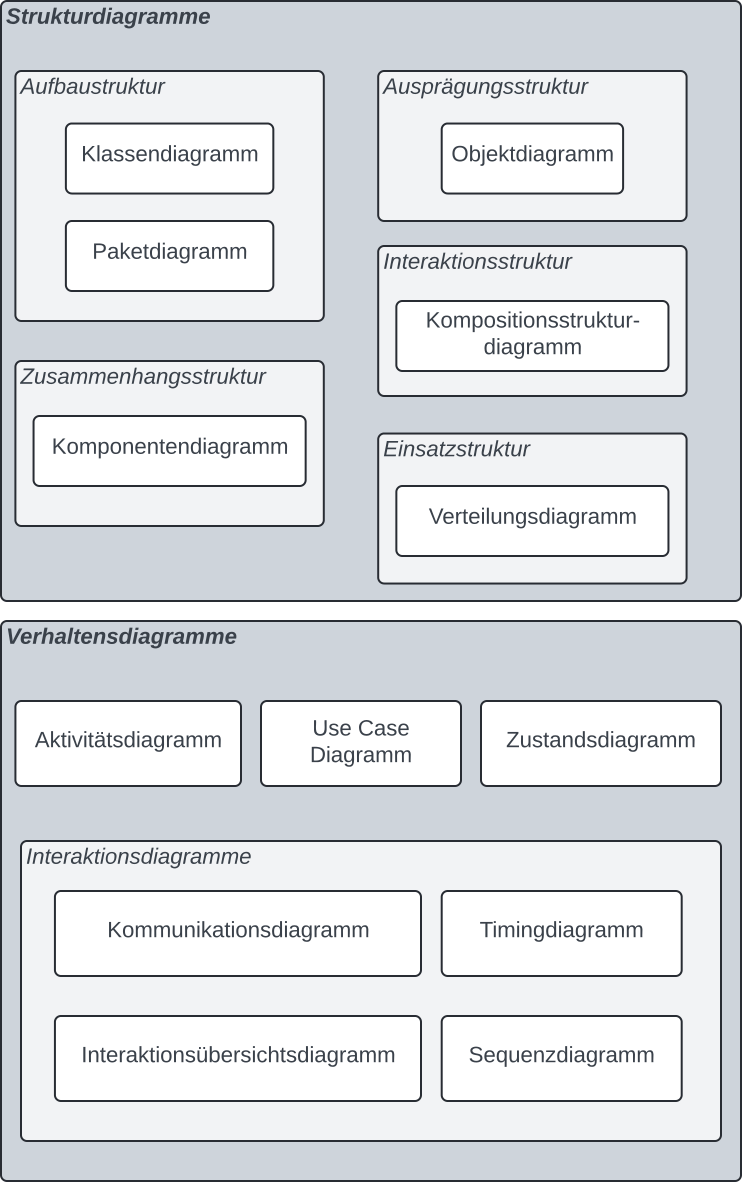
\includegraphics[scale=0.5]{part three/Einführung/img/diagrammübersicht}
    \caption{Diagrammübersicht nach \textit{Buhl}. (Quelle: in Anlehnung an \cite[7]{Buh09})}
    \label{fig:diagrammuebersicht}
\end{figure}

\subsection{Strukturdiagramme}
In den \textbf{Strukturdiagrammen} werden statische Strukturaspekte eines Systems betrachtet.
Für eine Systemmodellierung können alle dieser 6 Diagramme verwendet werden.

\begin{itemize}
    \item \textbf{Klassendiagramm}: Das \textbf{Klassendiagramm} wird verwendet, um ein objektorientiertes System zu beschreiben.
    \item \textbf{Paketdiagramm}: Ein \textbf{Paketdiagramm} zeigt die Pakete eines Systems und deren Beziehungen.\\
    Ein \textbf{Paket} gruppiert \textit{Modellelemente} (bspw. Klassen) unter Verwendung eines einheitlichen Namensraum: ``Das Konzept des Pakets wird benötigt, um die Elemente des Modells in sinnvoller Weise zu gruppieren und die Sytemstruktur auf einer hohen Abstraktionsebene zu beschreiben.`` (\cite[55]{Bal05})
    \item \textbf{Komponentendiagramm}: Stellt Komponenten oder auch \textit{Subsysteme} mit definierten Interfaces dar, um bspw. \textbf{Architekturdesign} darzustellen.
    \item \textbf{Verteilungsdiagramm}: Beschreibt eine Menge von Knoten, die die \textit{Ausführungsarchitektur} eines Systems definieren können, wobei Knoten i.d.R. \textit{Geräte} oder \textit{Softwareablaufumgebungen repräsentieren}.
    \item \textbf{Kompositionsstrukturdiagramm}: Stellt die \textbf{Komposition} von \textit{Systemstrukturen} (Klassen, Komponenten, Gesamtsystem) in einem bestimmten \textit{Kontext} mit einem bestimmten \textit{Ziel} dar (vgl. \cite[9]{Buh09}).
    \item \textbf{Objektdiagramm}: Momentaufnahme eines Systems zu genau einem \textit{Zeitpukt} während der Ausführung
\end{itemize}


\subsection{Verhaltensdiagramme}
\textbf{Verhaltensdiagramme} stellen \textit{Dynamik}, \textit{interne Abläufe} und das \textit{Zusammenspiel} der Systemteile dar, um eine Spezifikation zu vervollständigen.

\begin{itemize}
    \item \textbf{Anwendungsfalldiagramm}: Dienen zur \textit{Spezifizierung} und \textit{Formalisierung} von \textit{Systemanforderungen}, unter Berücksichtigung von \textbf{Akteuren}, \textbf{Systemen} und \textbf{Anwendungsfällen}
    \item \textbf{Zustandsdiagramm}: Auch \textbf{Zustandsautomaten}; zeigen für ein einzelnes Objekt Zustandsänderungen während der Lebenszeit
    \item \textbf{Aktivitätsdiagramme}: Werden zur Modellierung von \textit{Kontroll}- oder \textit{Objektflüssen} oder zur Darstellung von \textit{Programmlogik} genutzt.
    \item \textbf{Interaktionsdiagramme}: Stellen das Zusammenspiel mehrerer Kommunikationspartner dar.
    Es gibt unterschiedliche Typen von Interaktionsdiagrammen, die Interaktionen auf verschiedenen \textit{Abstraktionsebenen} modellieren:
    \begin{itemize}
        \item \textbf{Sequenzdiagramm}: Zeigt den Verlauf einer Interaktion in zwei Dimensionen, \textit{Kommunikationspartner} und die Nachrichten in ihrer \textit{zeitlichen Abfolge}
        \item \textbf{Kommunikationsdiagramm}: hebt die Kommunikationsbeziehungen zwischen den Partnern hervor
        \item \textbf{Timing Diagramm}: hebt die zeitlichen Aspekte einer Interaktion hervor
        \item \textbf{Interaktionsüberblickdiagramm}: Spezialfall des \textbf{Aktivitätsdiagramms} - statt Aktionen und Aktivitäten können das \textbf{Sequenz}-, \textbf{Kommunikations}- und das \textbf{Timing}-Diagramm als Knoten verwendet werden.
    \end{itemize}
    Alle verwenden dieselben Grundelemente: \textit{Lebenslinien} der Akteure und Nachrichten, die zwischen diesen ausgetauscht werden.

\end{itemize}
